\documentclass[a4paper]{article}

\usepackage[english]{babel}
\usepackage[utf8]{inputenc}
\usepackage{amsmath}
\usepackage{graphicx}
\usepackage[colorinlistoftodos]{todonotes}
\usepackage{xcolor} % note: there's also a color package instead of xcolor
\usepackage{verbatim}


%TODO

\begin{comment}
 Add background concepts
	use balanced ternary as an intro to probability current
Physical Implementations
Brief discussion of the different architectures
Discuss access of machines themselves
Discuss how to use code API such as QiSkit
Find a way to highlight comment begins and ends
replace emphasis in biblio with italix to fix the spacing issues

\end{comment}
%%%%%%%%%%%%%%%%%%%%%%%%%%%%%%%%%%%%%%%%%%
% Custom Defines
\definecolor{mygray}{gray}{0.6}
% Put a URL Define Here



%%%%%%%%%%%%%%%%%%%%%%%%%%%%%%%%%%%%%%%%%%
\title{A Brief introduction to Quantum Computing from the Perspective of Ladder Logic}

\author{Jerry Kensler}

\date{\today}

\begin{document}
\maketitle

\begin{abstract}

\begin{comment}
	%Reword this, it's  too boring
	
%Enter a short summary here. What topic do you want to investigate and why? What experiment did you perform? What were your main results and conclusion?
%

%Quantum computing, for several years the media and public perception of the subject has treated it akin to magic, using it as a catchall for any science fiction plot device deemed necessary.  Because of this, otherwise capable individuals may tend to stray away from the subject purely due to its perceived difficulty, many assuming they would need doctorates to even begin to comprehend the complexities of quantum computing.  Indeed, quantum physics is very complex, having many important real-world ramifications. With that said, quantum computing is merely a small part of quantum physics, and much like the computing most people use daily, operates by a well-defined set of rules.  By utilizing a subset of these rules, specifically tools such as quantum ladder logic, quantum assembly (QASM), and visual aids such as Bloch spheres, much of the initial barrier to entry can be circumvented.  While this approach isn’t perfect, and will require more serious individuals to pursue much of the background math and physics on their own.  It is my hope that students, specifically those with a background in electronic circuits and/or programming will find the contents of this paper able to greatly reduce the amount of time and effort needed in order to start learning how to program a quantum computer and thus prepare themselves for a future where such technology is prevalent.
\end{comment}

While Quantum Computing is a fairly advanced topic, it suffers from a perception of complexity beyond what is reasonable for the actual subject matter.  This paper provides a means to take that perception and bring it down to a more realistic level.  The primary targets of this paper are students currently enrolled in or freshly graduated from an electrical engineering or similar program; however, any individual with a base knowledge in programming or digital logic should be able to gain some level of benefit.

Keywords:  Quantum, QISKit, Computing, Ladder, Logic, QASM, Introduction
% Need to reword this section, Find the abstract from source and merge the two
% Author note: the intention of this paper is to fill some of the skill gap many novices encounter in learning quantum computing.  By no means should this be considered an all-encompassing guide to the subject matter.
\end{abstract}




\section{Introduction}
\label{sec:introduction}

%Explain the context of the experiment here. Why is condensed matter physics interesting or important?
%Optional things you could talk about (but don't have to -- this is up to you): transistors, computers, Quantum computers, fundamental knowledge (e.g. the resistance quantum).

%Briefly explain what methods you will use in the experiment, and what values you will extract from the data.

%For this section and all following sections: If you refer to an equation, previous result or theory that is not regarded as common knowledge, then cite the source (article or book) where you found this. For example, you can cite the Nano 3 Lecture notes \cite{nano3}.

This section is for context.  The how, and why.  From here on out, if I refer to a theory that isn't common knowledge, cite the source. \cite{junctNew}.


\section{Background Concepts}
\label{sec:backgroundconcepts}
%brief intro to this section, needs rewording
This section is not meant to be an exhaustive list, but, in my personal experience, learning about the background concepts below will greatly assist a person’s ability to better understand quantum computing.  The following sections will provide a brief explanation of the concepts.
\subsection{Balanced Ternary} %The basics from the ground up
%note: blanaced ternary is not, strictly speaking a core mechanic in quantum computing.  However, it could serve as a gentle introduction to non-binary coding for many students.  A bridge between hard digital and the strangeness of qubits
insert balanced ternary section here along with comparison table.

%\subsection{How to Make Tables}

Use the table and tabular commands for basic tables --- see Table~\ref{tab:widgets}, for example.

\begin{table} %Table used to illustrate comparison between bases
	\centering
	\begin{tabular}{l|l|l} % Justification l-left, c-center, r-right
		Decimal & Binary (IEEE 754*) & Balanced Ternary \\\hline %might remove the 754 example if it becomes an issue to clarity
		0 & 0 & 0 \\
		3 & 11 & 10 \\
		5 & 101 & + 0 - \\
		-254 & 11000011011111100000000000000000* & - 0 0 - + - \\ % -3^5 + 0 + 0 - 3^2 + 3^1 -3^0
	\end{tabular}
	\caption{\label{tab:widgets}comparison table showing equivalent numbers in different display forms}
\end{table}


\subsection{Reversible Logic Gates} %The basics from the ground up
%there was a time when reversible logic was seen as a fatal flaw in QC, but some dude who was pretty clever figured out any standard logic gate could be simulated within reversible logic
Talk about why reversible logic gates are important to quantum computing, a bit of the history, etc.


\section{Theory 2-3 pages}
\label{sec:theory}


\begin{comment} %comment out defaults
\subsection{Two-dimensional Electron Gas}
Here, explain the concept of a 2-DEG in GaAs/AlGaAs. What is a 2-DEG and why does it arise?

\subsection{Hall Effect}
Explain the classical Hall effect in your own words. What do I measure at $B=0$? And what happens if $B>0$? Which effect gives rise to the voltage drop in the vertical direction?

\subsection{Quantum Hall Effect}
Explain the IQHE in your own words. What does the density of states look like in a 2-DEG when $B=0$? What are Landau levels and how do they arise? What are edge states? What does the electron transport look like when you change the magnetic field? What do you expect to measure?

\end{comment}
\section{Experiment 1-2 pages}
\begin{comment} %comment out defaults
\subsection{Fabrication}
Explain a step-by-step recipe for fabrication here. How long did you etch and why? What is an Ohmic contact?
\subsection{Experimental set-up}
Explain the experimental set-up here. Use a schematic picture (make it yourself in photoshop, paint, ...) to show how the components are connected. Briefly explain how a lock-in amplifier works.

\end{comment} %comment out defaults

\section{Results and interpretation 2-3 pages}
Show a graph of the longitudinal resistivity ($\rho_{xx}$) and Hall resistivity ($\rho_{xy}$) versus magnetic field, extracted from the raw data shown in figure \ref{fig:data}. You will have the link to the data in your absalon messages, if not e-mail Guen (guen@nbi.dk). Explain how you calculated these values, and refer to the theory.

%\begin{figure}
%\centering
%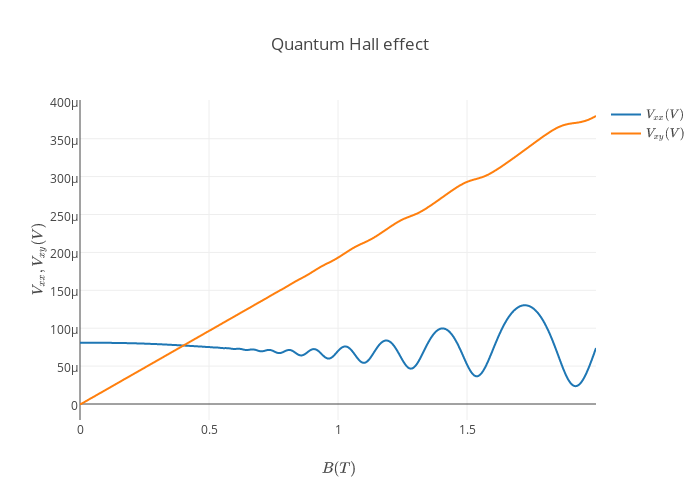
\includegraphics[width=1\textwidth]{raw_data.png}
%\caption{\label{fig:data}Raw (unprocessed) data. Replace this %figure %with the one you've made, that shows the resistivity.}
%\end{figure}
\begin{comment} %comment out defaults
\subsection{Classical regime}
Calculate the sheet electron density $n_{s}$ and electron mobility $\mu$ from the data in the low-field regime, and refer to the theory in section \ref{sec:theory}. Explain how you retrieved the values from the data (did you use a linear fit?).
Round values off to 1 or 2 significant digits: 8.1643 ~= 8.2. Also, 5e-6 is easier to read than 0.000005.

!OBS: This part is optional (only if you have time left).
Calculate the uncertainty as follows: \newline $u(f(x, y, z)) = \sqrt{(\frac{\delta f}{\delta{x}} u(x))^{2} + (\frac{\delta f}{\delta{y}} u(y))^{2} + (\frac{\delta f}{\delta{z}} u(z))^{2}}$, where $f$ is the calculated value ($n_{s}$ or $\mu$), $x, y, z$ are the variables taken from the measurement and $u(x)$ is the uncertainty in x (and so on).

\subsection{Quantum regime}
Calculate $n_{s}$ for the high-field regime.
Show a graph of the longitudinal conductivity ($\rho_{xx}$) and Hall conductivity($\rho_{xy}$) \textbf{in units of the resistance quantum} ($\frac{h}{e^{2}}$), depicting the integer filling factors for each plateau.
Show a graph of the plateau number versus its corresponding value of $1/B$. From this you can determine the slope, which you use to calculate the electron density.
Again, calculate the uncertainty for your obtained values.
\end{comment} %comment out defaults

\section{Discussion 1/2-1 page}
Discuss your results. Compare the two values of $n_{s}$ that you've found in the previous section. Compare your results with literature and comment on the difference. If you didn't know the value of the resistance quantum, would you be able to deduce it from your measurements? If yes/no, why?

\begin{comment} %comment out defaults

\newpage
\section{Some LaTeX tips}
\label{sec:latex}
\subsection{How to Include Figures}

First you have to upload the image file (JPEG, PNG or PDF) from your computer to writeLaTeX using the upload link the project menu. Then use the includegraphics command to include it in your document. Use the figure environment and the caption command to add a number and a caption to your figure. See the code for Figure \ref{fig:frog} in this section for an example.

%\begin{figure}
%\centering
%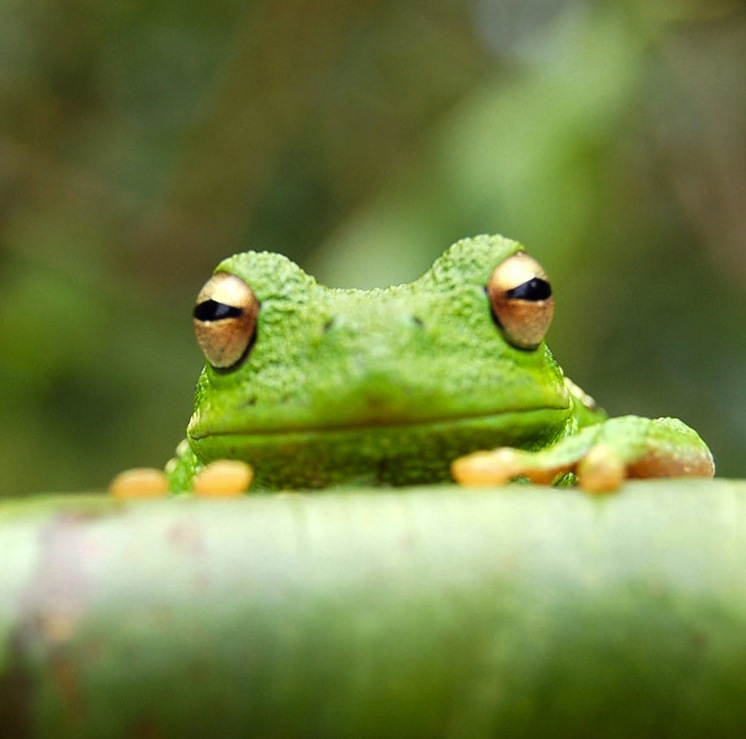
\includegraphics[width=0.3\textwidth]{frog.jpg}
%\caption{\label{fig:frog}This frog was uploaded to writeLaTeX via %the project menu.}
%\end{figure}



\subsection{How to Write Mathematics}

\LaTeX{} is great at typesetting mathematics. Let $X_1, X_2, \ldots, X_n$ be a sequence of independent and identically distributed random variables with $\text{E}[X_i] = \mu$ and $\text{Var}[X_i] = \sigma^2 < \infty$, and let

\begin{equation}
S_n = \frac{X_1 + X_2 + \cdots + X_n}{n}
      = \frac{1}{n}\sum_{i}^{n} X_i
\label{eq:sn}
\end{equation}

denote their mean. Then as $n$ approaches infinity, the random variables $\sqrt{n}(S_n - \mu)$ converge in distribution to a normal $\mathcal{N}(0, \sigma^2)$.

The equation \ref{eq:sn} is very nice.

\subsection{How to Make Sections and Subsections}

Use section and subsection commands to organize your document. \LaTeX{} handles all the formatting and numbering automatically. Use ref and label commands for cross-references.

\subsection{How to Make Lists}

You can make lists with automatic numbering \dots

\begin{enumerate}
\item Like this,
\item and like this.
\end{enumerate}
\dots or bullet points \dots
\begin{itemize}
\item Like this,
\item and like this.
\end{itemize}
\dots or with words and descriptions \dots
\begin{description}
\item[Word] Definition
\item[Concept] Explanation
\item[Idea] Text
\end{description}



We hope you find write\LaTeX\ useful, and please let us know if you have any feedback using the help menu above.


\end{comment} %comment out defaults


%%%%%%%%%%%%%%%%%%%%%%%%%%%%%%%%%%%%%%%%%%%%%%%%%%%%%%%%%%%%%%%%%%

\begin{thebibliography}{9}
	


\bibitem{junctNew}  
	Richard Newrock,
	\emph{"What are Joesphson Junctions? How do they work?"}
	Scientific American
	

\bibitem{mitqcshor}
	Shor, Peter. \emph{"Quantum Computation".} MIT OpenCourseware. Massachusetts Institute of Technology, 2003,18.435J / 2.111J / ESD.79J, \newline https://ocw.mit.edu/courses/mathematics/18-435j-quantum-computation-fall-2003/

\bibitem{cmuqc15}
	O'Donnell, Ryan. Wright, John. \emph{"Quantum Computation and Information".} Carnegie Mellon University, 2015, 15-859BB, \newline https://www.cs.cmu.edu/~odonnell/quantum15/

\bibitem{qazoo}
	Jordan, Stephan. \emph{"Quantum Algorithm Zoo".} National Institute of Standards and Technology (NIST),  https://math.nist.gov/quantum/zoo/
	
\bibitem{qiskit}
	QISKit. \emph{"QISKit."} https://github.com/QISKit. Accessed: February 14 2018
\begin{comment} % More info on QISKit
https://github.com/QISKit
  https://github.com/QISKit/ibmqx-user-guides
  https://github.com/QISKit/qiskit-tutorial
     https://github.com/QISKit/qiskit-tutorial/blob/master/INSTALL.md
        https://datascience.ibm.com/
        https://medium.com/qiskitters/qiskit-turns-one-looking-back-cbc2c48d7a95
     https://github.com/QISKit/qiskit-tutorial/blob/master/hello_world/quantum_emoticon.ipynb
\end{comment} % End QISKit extra info

\bibitem{qbenchgame}
	Wooten, James. \emph{"Using a Simple Puzzle Game to Benchmark Quantum Computers".} Medium, January 16 2018. https://medium.com/@decodoku/understanding-quantum-computers-through-a-simple-puzzle-game-a290dde89fb2

\begin{comment}% Further info on the benchmark game

https://mybinder.org/v2/gh/decodoku/A_Game_to_Benchmark_Quantum_Computers/master?filepath=Play_Quantum_Awesomeness.ipynb
    Also seen below, using a python game to illustrate quantum noise

https://medium.com/@decodoku/quantum-computation-in-84-short-lines-d9c7c74be0d0
    https://medium.com/@decodoku
        https://mybinder.org/v2/gh/decodoku/A_Game_to_Benchmark_Quantum_Computers/master?filepath=Play_Quantum_Awesomeness.ipynb
            Also seen above
\end{comment}% End further info on quantum benchmark game

\bibitem{algoassert} %finish this up
	Gidney, Craig. \emph{"Algorithmic Assertions"} Google AI, http://algassert.com/. Accessed: \date{\today}
\begin{comment} % helpful links on the site
http://algassert.com/quantum/2014/03/07/Building-your-own-Quantum-Fourier-Transform.html
	http://algassert.com/post/1704
		circuit width talk
	http://algassert.com/post/1628
		swapping to teleporting with simple circuit moves
	http://algassert.com/post/1618
		Affecting atoms by looking at emitted light
	http://algassert.com/quantum/2015/05/01/Quantum-Network-Flow-Puzzle.html
\end{comment} % End helpful links on the site


%========================================================================================

%\bibitem{template}
%	AuthorLast, AuthorF MI. \emph{"TitleOfSource.} OptionalCityOfPublication, OptionalDateOfOriginalPublication" TitleOfContainer. Version, OtherContributers, NumberSuchAsEpisodeVolume. Publisher, PublicationDate, LocationSuchAsPageNumberOrURL_Or_DOI. AccessedDayMonthSpelledOutYear

%https://owl.english.purdue.edu/owl/resource/747/01/

%========================================================================================

\begin{comment} %Start block comment


========Old Section=====

Gates: http://www.inetdaemon.com/img/gates.gif

https://inspirehep.net/record/1320783/files/fig1b.png


========================
===========Things Used=============

https://people.eecs.berkeley.edu/~vazirani/quantum.html



https://console.bluemix.net/dashboard/apps/
  This is Watson and other things


https://github.com/github/gitignore/blob/master/TeX.gitignore
  This is the gitignore settings nessisary to not constantly upload aux files when using LaTeX

http://web.mit.edu/rsi/www/pdfs/new-latex.pdf
  How to write in LaTeX

https://quantumexperience.ng.bluemix.net/qx/tutorial?sectionId=full-user-guide&page=introduction
	IBM Quantum Experience User guide
	https://quantumexperience.ng.bluemix.net/qx/community/question?questionId=e4b7b71ae47096a45e70fbcde8aee687
		A grover's algorithm implementation


http://paulklemm.com/blog/2014-07-16-use-github-for-scientific-writing/

https://arxiv.org/abs/1804.03719
	Quantum Algorithm Implementations for Beginners


https://quantumcomputing.stackexchange.com/
    --A place where people can ask questions and get help with quantum computing
    https://quantumcomputing.stackexchange.com/questions/1404/will-deep-learning-neural-networks-run-on-quantum-computers
	Will Neural Networks run on Quantum Computers

https://www.quantiki.org/wiki/basic-concepts-quantum-computation

https://www.media.mit.edu/quanta/qasm2circ/
	to draw circuits
https://tex.stackexchange.com/questions/9767/whats-a-good-package-for-typesetting-quantum-circuits

http://kim.oyhus.no/QuantumMechanicsForProgrammers.html


https://arxiv.org/pdf/1610.06980.pdf
	A paper on IBM Q that needs translation but looks relevant

https://arxiv.org/pdf/quant-ph/0308074.pdf
	Probability amplitute in Quantum-Like Games

https://arxiv.org/abs/1205.4926
	Quantum Delayed Choice Experiment

https://crypto.stackexchange.com/questions/3932/in-laymans-terms-how-does-shors-algorithm-work
	Prime Numbers: In layman's Terms, How does Shor's ALgorithm Work


https://www.quora.com/Is-it-possible-to-build-a-very-primitive-quantum-computer-at-home


https://arxiv.org/pdf/quant-ph/0503228v1.pdf
	The Physics of Factorization

https://arxiv.org/abs/1505.04577
	Analogue algorithm for parallell factorization of an exponential number of Large integers 1. Theoretical Description

http://stationq.github.io/Liquid/
	Language integrated Quantum Op Simulator
		Don't remember using, but it was with the links so I'll check on it later

https://kukuruku.co/post/quantum-circuits-methods-and-techniques/

https://hackaday.com/2017/01/24/the-birth-of-quantum-electrodynamics/

https://www.media.mit.edu/quanta/qasm2circ/

https://www.dwavesys.com/software



==========Stuff that is handy to have=============

http://backreaction.blogspot.com/2017/08/the-annotated-math-of-almost-everything.html?spref=tw

https://hackaday.com/2018/01/24/quantum-weirdness-in-your-browser/

Github Tutorial: 
  https://try.github.io/

https://www.overleaf.com/latex/templates/
  LaTeX Document templates for things like Resumes and Academic Reports

https://hackaday.com/2018/04/19/when-4-1-equals-8-an-advanced-take-on-pointers-in-c/
  A good tutorial on pointers in C



========================
==========Might use section==============
https://www.overleaf.com/latex/examples/title-page-with-logo/hrskypjpkrpd

https://github.com/adamisntdead/QuSimPy
  A quantum simulator someone wrote in python,  Could be useful to reference and see how they did things

Microsoft Q#
	https://docs.microsoft.com/en-us/quantum/?view=qsharp-preview
	https://docs.microsoft.com/en-us/quantum/quantum-writeaquantumprogram?view=qsharp-preview&tabs=tabid-vs2017
%
%============
%=========Extended Reading?================

%
%Data structure search visualization
%	https://visualgo.net/en
%
%
%https://www.nextplatform.com/2017/03/29/neuromorphic-quantum-supercomputing-mesh-deep-learning/
%
%https://arstechnica.com/science/2017/04/the-route-to-high-speed-quantum-computing-is-paved-with-error/
%
%https://drstienecker.com/tech-332/5-ladder-logic/
%
%https://www.youtube.com/user/LookingGlassUniverse/videos
%	videos on quantum computing and weirdness
%
%https://journals.aps.org/prl/abstract/10.1103/PhysRevLett.69.2881
%
%https://arxiv.org/abs/quant-ph/0006004
%	Fast paralell Circuits for the Quantum Fourier Transform
%
%https://www.nature.com/news/quantum-computers-ready-to-leap-out-of-the-lab-in-2017-1.21239
%
%https://www.youtube.com/watch?v=N6w9Pq6Q9OM
%	Spintronics Explanation
%
%=========Misc Helpful Links ===============
%
%news.ycombinator.com
%	Tech news
%
%hackaday.com
%	Various projects


  
%%%%EXAMPLE MLA FORMAT

%https://owl.english.purdue.edu/owl/resource/747/12/
%


%https://owl.english.purdue.edu/owl/resource/747/01/



\end{comment}
\end{thebibliography}
\begin{scriptsize}
\textcolor{mygray}{For extended reading list, consult source code, available at: \newline https://www.github.com/Macrofarad/ABriefIntroductionToQuantumComputingFromThePerspectiveOfLadderLogic}

%Edit as url changes, suggest placing completed project as new repository with a slightly better name
\end{scriptsize} %size list: Huge, huge, LARGE, Large, large, normalsize, small, footnotesize, scriptsize, tiny
\end{document}
